\chapter{Referencial teórico}

O referencial teórico revela o momento de levantar o embasamento teórico sobre o tema de pesquisa. No contexto desse TCC, faz-se necessário, dentros outros aspectos pesquisar sobre os entendimentos existentes do problema de pesquisa e analisar quais mecanismos devem ser adotados para se propor uma solução \cite{belchior2012}.

O referencial teórico deste TCC irá levantar o embasamento teórico sobre Contexto Financeiro, Métodos Matemáticos, Paradigmas de Programação e Testes estáticos/dinâmicos para que seja possível propor uma solução para o problema de pesquisa.

\section{Contexto Financeiro}
Esta seção irá tratar os atributos aliados ao contexto financeiro como Alavancagem, Suporte e Resistência. Esses atributos são insumos para que se possa compreender melhor a dinâmica das estratégias para negociação no Mercado de Moedas.

\subsection{Mercado de Moedas}
Mercado de Moedas ou FOREX (abreviatura de Foreign Exchange) é um mercado interbancário onde as várias moedas do mundo são negociadas. O FOREX foi criado em 1971, quando a negociação internacional transitou de taxas de câmbio fixas para flutuantes. Com o resultado do seu alto volume de negociações, o Mercado de Moedas tornou-se o principal mercado financeiro do mundo \cite{market2011}.

A operação no Mercado de Moedas envolve a compra de uma moeda e a simultânea venda de outra. As moedas são negociadas em pares, por exemplo: euro e dólar (EUR-USD). O investidor não compra ou vende euro e dólares fisicamente, mas existe uma relação monetária de troca entre eles. O FOREX é um mercado em que são negociados, portanto, derivativos de moedas. O investidor é remunerado pelas diferenças entre a valorização (se tiver comprado) ou desvalorização (se tiver vendido) destas moedas \cite[p.~3]{cvm2009}.

O Mercado de Moedas é descentralizado, pois as operações são realizadas por vários participantes do mercado em vários locais. É raro uma moeda manter uma cotação constante em relação a outra moeda. O câmbio entre duas moedas muda constantemente \cite[p.~5]{fxcm2011}.

O Mercado de Moedas é constituído por transações entre as corretoras que operam no mesmo e são negociados, diariamente, contratos representando volume total entre 1 e 3 trilhões de dólares. As transações são realizadas diretamente entre as partes (investidor e corretora) por telefone e sistemas eletrônicos, desde que tenham conexão à internet. As operações ocorrem 24 horas por dia, durante 5 dias da semana (abrindo às 18h no domingo e fechando às 18h na sexta; horário de Brasília), negociando os principais pares de moedas, ao redor do mundo \cite[p.~4]{cvm2009}.

\subsection{Alavancagem}
Alavancagem no contexto de mercado,deriva do significado de alavanca na Física, relacionado com a obtenção de um resultado final maior do que ao esforço empregado \cite[p.~3]{dantas2006}.

\begin{citacao}
O conceito de alavancagem é similar ao conceito de alavanca comumente empregado em física. Por meio da aplicação de uma força pequena no braço maior da alavanca, é possível mover um peso muito maior no braço menor da alavanca \cite[p.~232]{bruni2011}.
\end{citacao}

A Alavancagem possui a propriedade de gerar oportunidades financeiras para empresas que possuem indisponibilidade de recursos internos e/ou próprios \cite[p~13]{albuquerque2013}.

No mercado FOREX, o investidor pode negociar contratos de taxas de câmbio e usar a Alavancagem para aumentar suas taxas de lucro. Se o investidor, por exemplo, realizar uma operação de compra apostando 0.01 por ponto e o mercado subir 1000 pontos, ele ganha 10 dólares (0.001x1000). Usando a técnica de Alavancagem, o investidor pode realizar a mesma operação de compra colocando sua operação alavancada a 1.0, realizando o lucro de 1000 dólares (1.0x1000) \cite{easyforex2014}.

\subsection{Suporte}

Segundo \citeonline[p.~22]{matsura2006},  Suporte é o nível de preço no qual a pressão compradora supera a vendedora e interrompe o movimento de baixa. Pode-se identificar o Suporte por uma linha reta horizontal conforme a figura \ref{retaSuporte}.

\begin{figure}
\centering
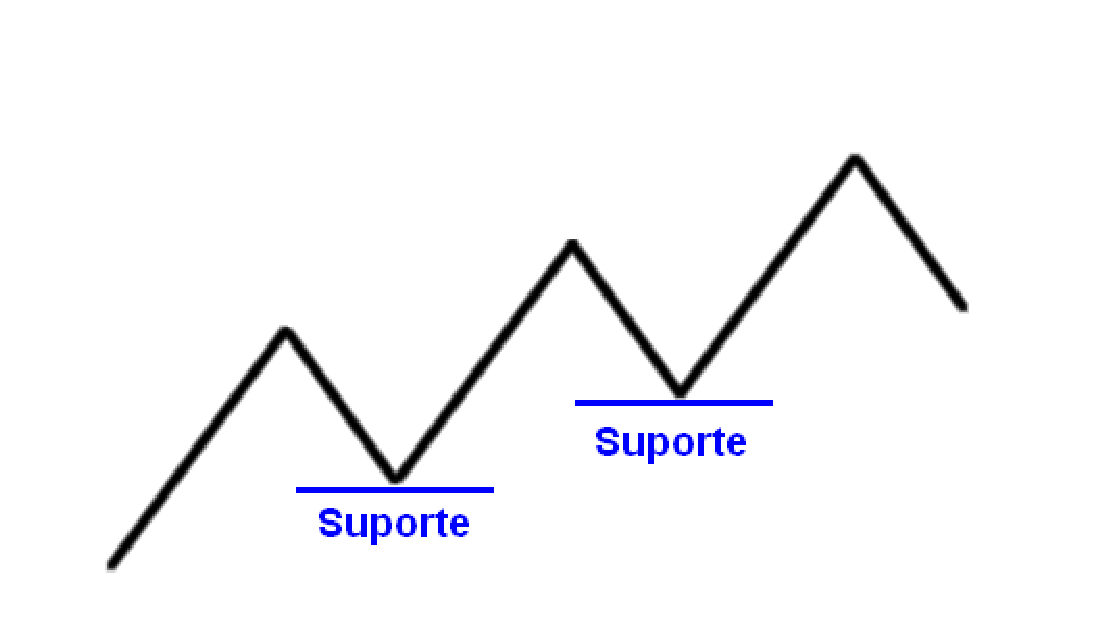
\includegraphics[width=0.9\textwidth]{figuras/retaSuporte}
\caption{Reta de Suporte.}{Fonte \citeonline[p.~22]{matsura2006}.}
\label{retaSuporte}
\end{figure}

Suporte é uma região gráfica que após uma queda, os preços param e revertem no sentido contrário. É uma área em que os investidores tendem a comprar \cite[p~97]{debastini2008}.

